\documentclass{article}
\usepackage{graphicx}
\usepackage[margin=1.5cm]{geometry}
\usepackage{amsmath}

\begin{document}

\title{Tuesday Reading Assessment: Unit 3, Magnetic Forces and Fields}
\author{Prof. Jordan C. Hanson}

\maketitle

\section{Memory Bank}

\begin{itemize}
\item $\vec{F} = q\vec{v} \times \vec{B}$ ... The Lorentz force, one version.
\item $\vec{F} = i\vec{L} \times \vec{B}$ ... The Lorentz force, another version.
\item $\vec{\tau} = \vec{r} \times \vec{F}$ ... Definition of torque.
\item $\vec{\tau} = \vec{\mu} \times \vec{B}$ ... Torque on a current carrying loop in a uniform B-field.
\item $\vec{\mu} = Ni\vec{A}$ ... Definition of the magnetic moment.
\end{itemize}

\section{The Power Generator}

\begin{enumerate}
\item Consider Fig. \ref{fig:lorentz}, in which a DC power generator is depicted inside a 0.05 T B-field.  Suppose the area of the loop is $10^{-2}$ m$^{2}$, the voltage in the circuit is 24 V, and the circuit resistance is 50 $\Omega$.  Also assume that there is just one loop of wire in the rotor.  What is the \textit{maximum torque} the system could achieve? \\ \vspace{2cm}
\begin{figure}[ht]
\centering
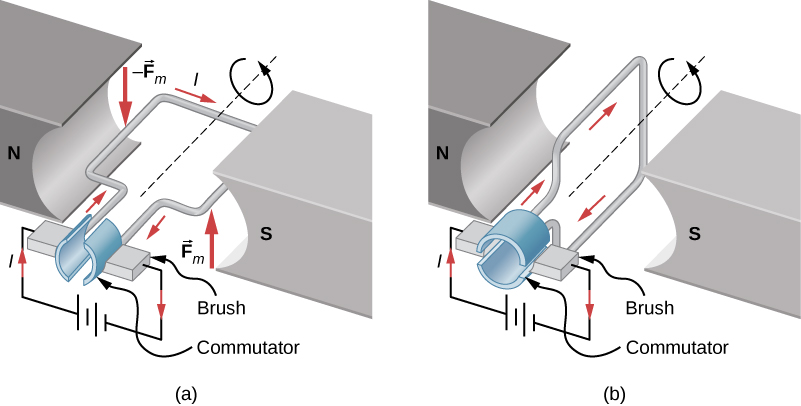
\includegraphics[width=0.55\textwidth]{commute.jpeg}
\caption{\label{fig:lorentz} An illustration of how a power generator works.  This version uses DC current and a commutator.}
\end{figure}
\item What would the maximum torque be if there were $N = 100$ turns of wire?
\end{enumerate}

\end{document}
